\documentclass[10pt,aspectratio=169]{beamer}

\mode<presentation>
{
    \usetheme[sectionpage, subsectionpage]{RTG2583}
}

% Standard packages
\usepackage[T1]{fontenc}
\usepackage[utf8]{inputenc}
\usepackage{lmodern}
\usepackage{microtype}
\usepackage{amsmath, amsfonts, amssymb, amsthm}
\usepackage[justification=centering]{caption} %
\captionsetup[figure]{labelformat=empty}% redefines the caption setup of the figures environment in the beamer class.
\captionsetup{belowskip=0pt}

\usepackage{hyperref}
\definecolor{my_blue}{RGB}{0,80,200} % 0,77,128
\hypersetup{%
    citecolor     = my_blue,% Color of citations % 
    urlcolor      = my_blue,%  Color of external urls, i used my_lightblue before
}
\usepackage{enumerate}
\usepackage[export]{adjustbox}
\usepackage{multimedia}
\usepackage{dsfont} % for indicator function 
\usepackage{caption}
\usepackage{subcaption}
\usepackage{soul} % strikethrough text
\usepackage{biblatex}
\addbibresource{literature.bib}
% Custom commands
\usepackage{algcompatible} % for long algorithms, algorithmicx
\usepackage{algorithm} % for algorithms
% \usepackage[symbol]{footmisc}
\usepackage{array} % draw matrices
\newcommand*{\vertbar}{\rule[-.5ex]{0.5pt}{5ex}}
\newcommand*{\horzbar}{\rule[.5ex]{5ex}{0.5pt}}
\usepackage{booktabs} % for fancy tables
\newcommand{\deriv}{\mathrm{d}} % new command for derivative d
\newcommand{\vect}[1]{\boldsymbol{#1}} % for bolding x 
\usepackage{tikz} % to create pictures 
\usetikzlibrary{positioning,shapes,arrows.meta}
\tikzset{
    process1/.style={rectangle, rounded corners, minimum width=4cm, minimum height=2cm, text width=8cm,text centered, draw=black, fill=red!30},
    process2/.style={rectangle, rounded corners, minimum width=4cm, minimum height=2cm, text width=5cm,text centered, draw=black, fill=orange!30},
    process3/.style={rectangle, rounded corners, minimum width=4cm, minimum height=2cm, text width=5cm,text centered, draw=black, fill=green!30},
    arr/.style={thick,-stealth}
    } % for the flow chart
%Title setup
\title[PhD project]{Technical Talk - PhD Project}
\subtitle{}
\author[Kamal Sharma]{Kamal Sharma}
\institute[UHH]{Department of Mathematics, University of Hamburg}

\date{February 13, 2026}


% Start document
\begin{document}
\begin{frame}[noframenumbering]
    \maketitle    
\end{frame}
\section{Introduction}
\begin{frame}{What is it about?}
\onslide<1->{\large \textcolor{teal}{Development} of a \textcolor{purple}{structure-preserving} \textcolor{orange}{idealized} \textcolor{orange}{stochastic climate model}
\vspace{5mm}
\begin{itemize}
    \item \textcolor{orange}{Climate model:} set of equations modelling coupled ocean-atmosphere dynamics
    \vspace{0.2cm}
    \item \textcolor{orange}{Idealized:} 2D model $\rightarrow$ solves for velocity, temperature, and pressure
    \vspace{0.2cm}
    \item \textcolor{orange}{Stochastic:} has stochastic/random terms (think of Brownian motion)
    \vspace{0.2cm}
    \item \textcolor{purple}{Structure-preserving:} preserves underlying geometric and physical structure
    % \item<6-> \textcolor{teal}{Development:} modeling, analysis, and \textcolor{teal}{simulation}
\end{itemize} 
\vspace{.5cm}}
\onslide<2>{\large \textbf{We are solving stochastic PDEs which model ocean-atmosphere interactions!}}
\end{frame}
\subsection{Why add stochastic terms?}
\begin{frame}{Multiscale phenomena}
    \begin{figure}
        \centering
        \includegraphics[width=0.35\linewidth]{images/multiscale_pheno.pdf}
        \vspace{-.3cm}
        \caption{Spatial and temporal scales of various meteorological phenomena\footfullcite{stullPracticalMeteorologyAlgebrabased2017}}
    \end{figure}
\begin{itemize}
    \onslide<1->{
    % \item Earth's oceans and atmosphere are characterized by a rich hierarchy of interacting processes
    % \vspace{-.4cm}
    \item Numerical models have fixed resolution
    \item Processes occurring below the model resolution are not captured $\rightarrow$ leads to prediction error!}
    \item<2-> \textbf{Solution}: Parameterization or subgrid-scale modeling
\end{itemize}
\end{frame}
\begin{frame}{Parameterization}
\begin{itemize}
    \item<1-> Additional terms are added to account for the missing effect of unresolved/small scales
    \item<1-> Parameterization techniques can be divided into two categories:
    \begin{enumerate}
        \item<1-> Deterministic
        \item<1-> Stochastic
    \end{enumerate}
    % \vspace{.2cm}
    \item<1-> We explored \textbf{stochastic parameterization} : {stochastic advection by Lie transport} (SALT)
    \vspace{.3cm}
    \item<2-> Why {SALT}? 
    % \begin{itemize}
        \item<2-> \textcolor{rtg_darkblue}{preserves conservation properties} $\rightarrow$ reliable long simulations
        \item<2-> \textcolor{rtg_darkblue}{better forecast skills} $\rightarrow$ uncertainty due to unresolved transport processes can be quantified
        \item<2-> conducive to \textcolor{rtg_darkblue}{data-driven approaches} $\rightarrow$ can be estimated from observations/satellite data
    % \end{itemize}
    % \item<4-> The stochastic terms models the unresolved transport processes! 
\end{itemize}
\end{frame}
\section{Research objectives}
\begin{frame}{Main objectives}
\begin{enumerate}
    \onslide<1->{
    \item Explore the efficacy of stochastic parameterization (in terms of UQ skills) for a climate model
    \begin{itemize}
        \item Previous studies focused on Euler, quasi-geostrophic, and shallow water equations
    \end{itemize}
    \vspace{.5cm}
    \item Numerically solve the idealized stochastic climate model}
    % \vspace{.2cm}
    % \item \only<1> {How to model the noise/stochastic term effectively?}
    % \only<2> {\st{How to model the noise/stochastic term effectively?}}
    % % \begin{itemize}
    % %     \item Are there better ways to calibrate the stochastic model?
    % % \end{itemize}
    % \vspace{.2cm}
    % \item \only<1> {Compare the stochastic model results with other existing models/approaches}
    % \only<2> {\st{Compare the stochastic model results with other existing models/approaches}}
\end{enumerate}    
\end{frame}
\section{The climate model}
\begin{frame}{Model equations}
  2D climate model equations:
\begin{columns}[T] % align columns
\begin{column}{.70\textwidth}
    \begin{footnotesize}
    \begin{align*}
            \text{Atmosphere}: \ &\deriv \mathbf{u}^a + ((\mathbf{u}^a \deriv t + \textcolor{violet}{\sum_i \boldsymbol{\xi}_i \circ \deriv W^i})\cdot \nabla) \mathbf{u}^a + \frac{1}{Ro^a} \hat{\mathbf{z}} \times (\mathbf{u}^a\deriv t + \textcolor{violet}{\sum_i \boldsymbol{\xi}_i \circ \deriv W^i}) \\
                &\quad \quad + \textcolor{violet}{\sum_i (u_1^a \nabla \xi_{i,1} + u_2^a \nabla \xi_{i,2} )\circ \deriv W^i} = (-\frac{1}{C^a} \nabla \theta + \frac{1}{Re^a} \Delta \mathbf{u}^a) \deriv t, \\
        &\deriv \theta^a + \nabla\cdot(\theta^a (\mathbf{u}^a\deriv t + \textcolor{violet}{\sum_i \boldsymbol{\xi}_i \circ \deriv W^i})) = (\textcolor{brown}{\gamma(\theta^a - \theta^o)} + \frac{1}{Pe^a} \Delta \theta^a )\deriv t,
        \end{align*}
        \begin{align*}
        \text{Ocean}: \ &\frac{\partial \mathbf{u}^o}{\partial t} + (\mathbf{u}^o\cdot \nabla)\mathbf{u}^o + \frac{1}{Ro^o} \hat{\mathbf{z}} \times \mathbf{u}^o + \frac{1}{Ro^o} \nabla p^a = \textcolor{brown}{\sigma(\mathbf{u}^o - \mathbb{E}\mathbf{u}_{sol}^a)} + \frac{1}{Re^o} \Delta \mathbf{u}^o,\\
            & \nabla \cdot \mathbf{u}^o = 0,\\
            &\frac{\partial \theta^o}{\partial t} + \mathbf{u}^o \cdot \nabla \theta^o = \frac{1}{Pe^o} \Delta \theta^o.
    \end{align*}
    \end{footnotesize}
% \item Our goal is to numerically solve the model equations!
% \end{itemize}
% \vspace{.2cm}
% Incompressible/compressible Navier-Stokes + Advection-diffusion eqs.
\end{column}%
\hfill%
\begin{column}{.30\textwidth}
% \vspace{.5cm}
\onslide<1->{
\begin{figure}
    \centering
    \includegraphics[width=1\linewidth]{images/domain.pdf}
    \caption{Model domain}
\end{figure}
$\mathbf{u}:$ velocity, \\ $\theta:$ temperature, \\ $p:$ pressure}
\end{column}%
\end{columns}
\vspace{.4cm}
Incompressible/compressible Navier-Stokes + Advection-diffusion equations
\end{frame}
\begin{frame}
    \frametitle{How to get the stochastic terms?}
    \begin{itemize}
        \onslide<1->{
        \item Difference between Lagrangian trajectories at different resolutions:
        $$\textcolor{violet}{\sum_i \boldsymbol{\xi}_i ~ \deriv W^i} \approx \mathbf{u}_{true}~\deriv t - {\mathbf{u}}~ \deriv t$$ $\mathbf{u}_{true}:$ true velocity \\
    ${\mathbf{u}}:$ mean flow velocity i.e. the large-scale component of $\mathbf{u}_{true}$
    \vspace{.5cm}
    \item Ways to estimate the true velocity $\mathbf{u}_{true}$:
    \begin{enumerate}
        \item Observation data (for example, from satellites)
        \item Synthetic data (from high-resolution numerical simulations)
    \end{enumerate}
    \vspace{.5cm}}
    \onslide<2->{
    \item \textbf{We use synthetic data (proof of concept)!}}
    \end{itemize}
\end{frame}
\begin{frame}{Our methodology}
\begin{figure}
    \centering
    \resizebox{1\textwidth}{!}{
        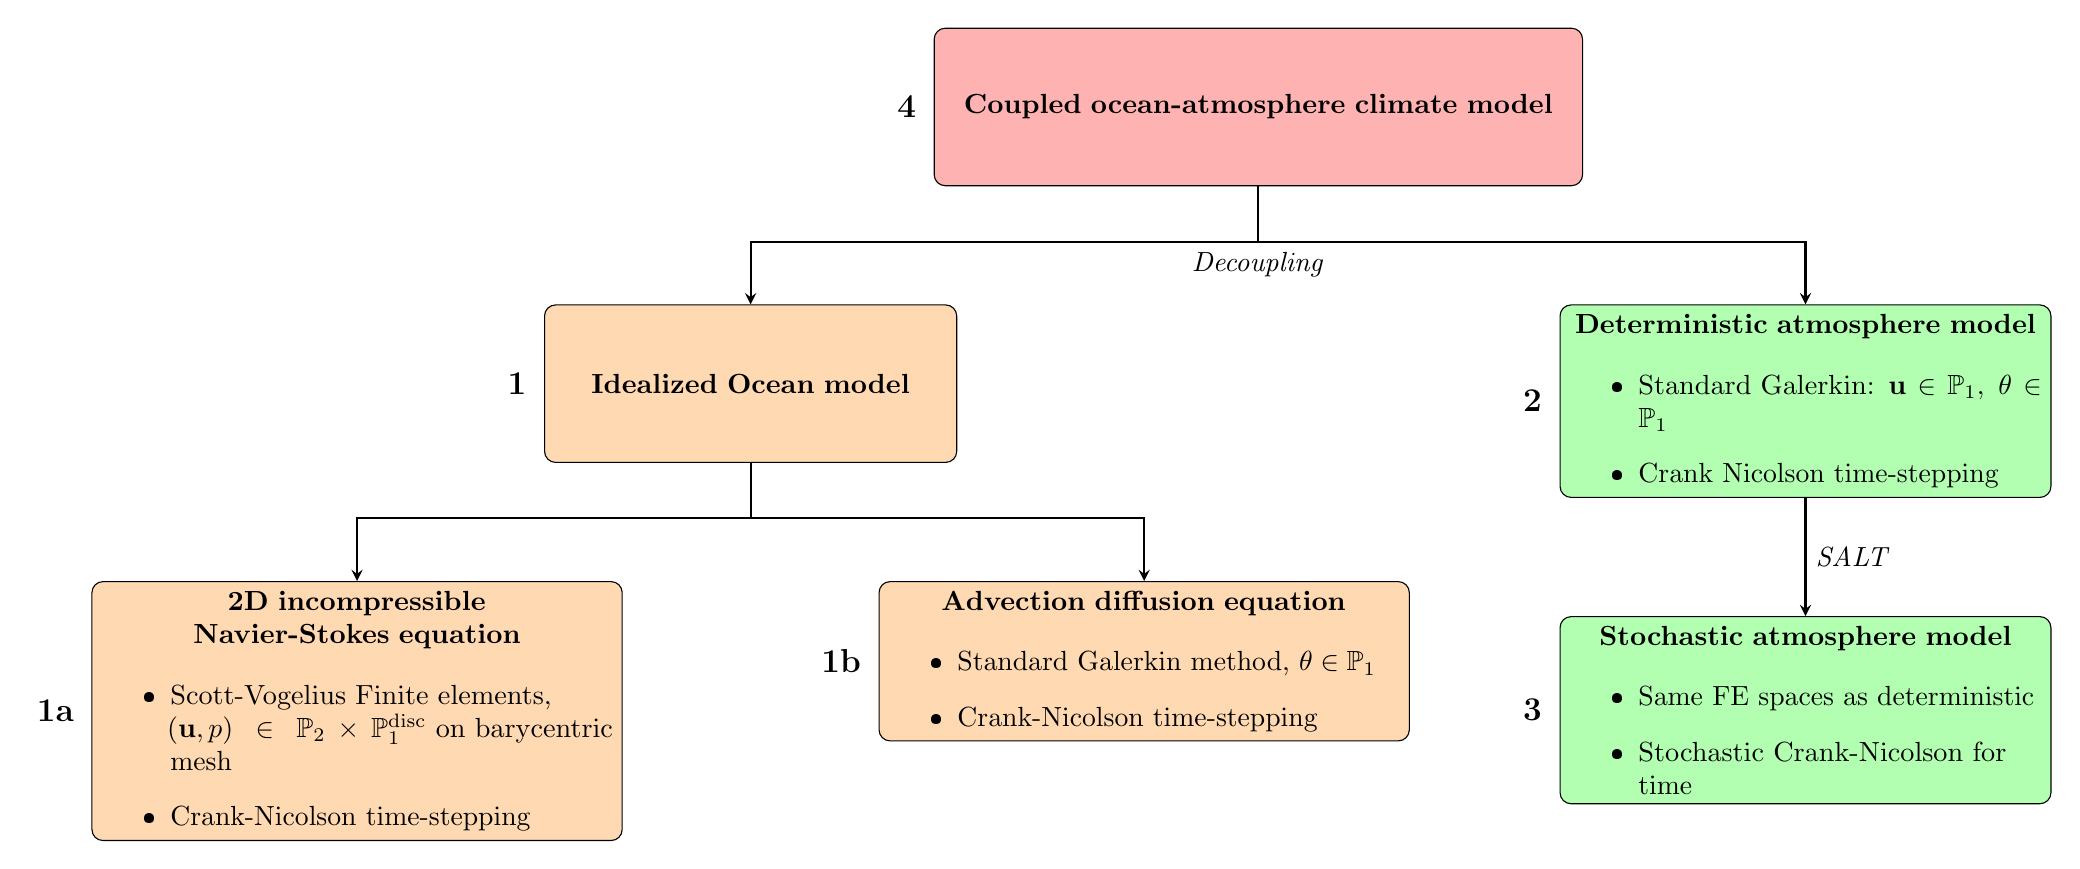
\begin{tikzpicture}[node distance=1cm]
        \node[process1] (main) {\textbf{Coupled ocean-atmosphere climate model}};
        \node[left = of main, xshift=.9cm] {\large{\textbf{4}}};
        \node[below left =1.5cm and -.3cm of main,process2,text width=5cm] (ocean) {\textbf{Idealized Ocean model}};
        \node[left = of ocean, xshift=.9cm] {\large{\textbf{1}}};
        \node[below right =1.5cm and -.3cm of main,process3,text width=6cm] (atmo) {\textbf{Deterministic atmosphere model}\\
        \begin{itemize}
            \item Standard Galerkin: $\mathbf{u} \in \mathbb{P}_1,~ \theta \in \mathbb{P}_1 $
            \item Crank Nicolson time-stepping
        \end{itemize}
        };
        \node[left = of atmo, xshift=.9cm] {\large{\textbf{2}}};
        \node[below left = 1.5cm and -1cm of ocean,process2,text width=6.5cm] (NS) {\textbf{2D incompressible Navier-Stokes equation} \\
        \begin{itemize}
            \item Scott-Vogelius Finite elements, $(\mathbf{u},p) \in \mathbb{P}_2\times\mathbb{P}_{1}^{\text{disc}}$ on barycentric mesh
            \item Crank-Nicolson time-stepping
        \end{itemize}};
        \node[left = of NS, xshift=.9cm] {\large{\textbf{1a}}};
        \node[below right = 1.5cm and -1cm of ocean,process2,text width=6.5cm] (adv) {\textbf{Advection diffusion equation}\\
        \begin{itemize}
            \item Standard Galerkin method, $\theta \in \mathbb{P}_1$
            % \item Spurious oscillations $\rightarrow$ adjust diffusion coefficient according to mesh
            \item Crank-Nicolson time-stepping
            \end{itemize}};
        \node[left = of adv, xshift=.9cm] {\large{\textbf{1b}}};
        % \node[below = of NS,process2, yshift=-.02cm, text width=6.5cm] (stoNS) {\textbf{Stochastic Navier-Stokes equations} \\ 
        % \begin{itemize}
        %     \item Model calibration
        %     \item Uncertainty quantification
        % \end{itemize}};
        % \node[left = of stoNS, xshift=.9cm] {\large{\textbf{3}}};
        \node[below = of atmo,process3, yshift=-.5cm,text width=6cm] (sto_atmo) {\textbf{Stochastic atmosphere model}\\
        \begin{itemize}
            \item Same FE spaces as deterministic
            \item Stochastic Crank-Nicolson for time
        \end{itemize}};
        \node[left = of sto_atmo, xshift=.9cm] {\large{\textbf{3}}};
    
        \draw[arr] (main.south) --++ (0,-20pt) -| (ocean) node[pos=0.0,below]{\textit{Decoupling}};
        \draw[arr] (main.south) --++ (0,-20pt) -| (atmo);
        \draw[arr] (ocean.south) --++ (0,-20pt) -| (NS);
        \draw[arr] (ocean.south) --++ (0,-20pt) -| (adv);
        % \draw[arr] (NS) -- node[anchor=west] {\textit{SALT}} (stoNS);
        \draw[arr] (atmo) -- node[anchor=west] {\textit{SALT}} (sto_atmo);
    \end{tikzpicture}
    }
    \end{figure}
    Incremental validation approach - solve simpler components first, verify at each step!
    % We used an open-source Python Finite Element package for numerical implementation and simulation
\end{frame}
\section{Numerical simulation of the climate model}
\begin{frame}{Data collection and model calibration}
\begin{itemize}
    \item We run the deterministic climate model in high-res. ($\Delta x = 1/128 \sim 30 ~ \text{km}$) % for 45 time units ($\sim 25 ~ \text{days}$)
    \vspace{-.3cm}
    \begin{figure}
    \captionsetup[subfigure]{labelformat=empty}
    \centering
    % First image
    \begin{subfigure}{1\textwidth}
        \centering
        \caption{Initial condition}
        \includegraphics[width=0.7\linewidth]{images/cm_t0.png}   
    \end{subfigure}
    \vspace{-.1cm}
    % Arrow between images
    \tikz[yshift=3pt]\draw[ thick,->] (0,0) -- ++(0,-0.25);
    % \tikz[yshift=5pt]\draw[thick,->] 
    % (0,0) -- ++(0,-0.5) node[midway,right]{After 45 time units};
    % Second image
    \begin{subfigure}{1\textwidth}
        \centering
        \caption{At t=45}
        \includegraphics[width=0.7\linewidth]{images/cm_t45.png}
    \end{subfigure}
    \end{figure}
    \item Analyze data $\rightarrow$ extract small-scale features (using statistical algorithms) $\rightarrow$ obtain $\textcolor{violet}{\sum_i \boldsymbol{\xi}_i ~ \deriv W^i}$
    \end{itemize}
\end{frame}
\subsection{Stochastic model simulation}
\begin{frame}{Stochastic model simulation}
\begin{itemize}
    \item We run the stochastic model on a coarse grid ($\Delta x = 1/32 ~ \sim 120 ~ \text{km}$) 
    \item Initial conditions correspond to coarse grained velocity and temperature fields at $t=25$ 
\end{itemize}
\begin{figure}
    \centering
    \begin{subfigure}[b]{\textwidth}
        \centering
        \includegraphics[width=0.45\linewidth]{images/cg_atm_temp_t25.pdf}
        \includegraphics[width=0.45\linewidth]{images/cg_atm_vel_t25.pdf}
    \end{subfigure}
    \begin{subfigure}[b]{\textwidth}
        \centering
        \includegraphics[width=0.45\linewidth]{images/cg_ocean_temp_t25.pdf}
        \includegraphics[width=0.45\linewidth]{images/cg_ocean_vel_t25.pdf}
    \end{subfigure}
\end{figure} 
% \item Atmospheric vorticity at $t=25$:
\begin{figure}
    \centering
    \caption{Atmospheric vorticity at $t=25$}
    % \vspace{-.4cm}
    \includegraphics[width=0.5\linewidth]{images/cg_atm_vort_t25.pdf}
\end{figure}
\end{frame}
\begin{frame}{Simulation results}
\begin{itemize}
    \item Stochastic model is simulated for 20 time units ($t=25$ to $t=45$)
    % \item 53 $\boldsymbol{\xi}_i$ out of 500 (which explains 99 $\%$ of the total variance) are used
    \item Stochastic vs. deterministic (without parameterization) model results at $t=35$
\end{itemize}
\vspace{-.5cm}
\begin{columns}[T] % align columns
\begin{column}{.48\textwidth}
        \begin{figure}
        \captionsetup[subfigure]{labelformat=empty}
            \centering
            \begin{subfigure}[b]{.85\textwidth}
            \caption{Particle 1}
            % \vspace{-.2cm}
            \includegraphics[width=1\linewidth]{images/vort_stoch_p1_same_99_var_ic_at_t35.pdf}
            \end{subfigure}
            \vspace{.2cm}
            \begin{subfigure}[b]{.85\textwidth}
            \caption{Particle 2}
            % \vspace{-.2cm}
            \includegraphics[width=1\linewidth]{images/vort_stoch_p2_same_99_var_ic_at_t35.pdf}
            \end{subfigure}
            \vspace{.2cm}
            \begin{subfigure}[b]{.85\textwidth}
            \caption{Particle 3}
            % \vspace{-.2cm}
            \includegraphics[width=1\linewidth]{images/vort_stoch_p3_same_99_var_ic_at_t35.pdf}
            \end{subfigure}
        \end{figure}
\end{column}%
\hfill%
\begin{column}{.48\textwidth}
        \begin{figure}
        \captionsetup[subfigure]{labelformat=empty}
            \centering
            \begin{subfigure}[b]{.85\textwidth}
            \caption{Deterministic sol. (w/o parameterization)}
            % \vspace{-.2cm}
            \includegraphics[width=1\linewidth]{images/vort_det_same_ic_at_t35.pdf}
            \end{subfigure}
            \vspace{.2cm}
            \begin{subfigure}[b]{.85\textwidth}
            \caption{\textbf{True solution}}
            % \vspace{-.2cm}
            \includegraphics[width=1\linewidth]{images/vort_truth_at_t35.pdf}
            \end{subfigure}
        \end{figure}
\end{column}%
\end{columns}
\end{frame}
\begin{frame}{Simulation results}
    \begin{itemize}
        \item<1-> Comparison between the stochastic ($\mu$ $\pm ~1 \sigma$) and deterministic sol. at 6 grid points:
        \onslide<1->{\begin{figure}
        \centering
        \caption{\textbf{Atmospheric velocity }($x$ component)}
        \vspace{-.2cm}
        \includegraphics[width=0.7\linewidth]{images/cm_res_32_atm_ux_var_99_part_50_t25_onwards_ppt.pdf}
        \end{figure}}
    \end{itemize} 
        \begin{enumerate}
            \item<1-> Ensemble spread increases over time
            \item<1-> Stochastic model captures the truth for 5 to 10 time units
        \end{enumerate}
    
\end{frame}
\begin{frame}{Uncertainty quantification}
    \begin{itemize}
        \item Plots for the evolution of ensemble spread and RMSE at six different locations on the grid
        \begin{figure}
        \centering
        \caption{\textbf{RMSE vs. spread} for $u^a_x$}
        \vspace{-.2cm}
        \includegraphics[width=0.65\linewidth]{images/spread_rmse_res_32_atm_ux_var_99_part_50_t25_onwards_ppt.pdf}
        \end{figure}
        \item Ensemble spread $\propto$ RMSE (for at least 15 time units)
        \item Error in the stochastic solution can be estimated by its own spread 
        % \begin{itemize}
        %     \item SPDE solution is suitable for data assimilation methods!
        % \end{itemize}
    \end{itemize}
\end{frame}
\section{Summary}
    \begin{frame}{Summary \& outlook}
    \begin{itemize}
        \item \textcolor{rtg_darkblue}{Aim:} solve a stochastic coupled ocean-atmosphere climate model
        \vspace{.2cm}
        \item \textcolor{rtg_darkblue}{Novelty:} data-driven model
        \begin{itemize}
            \item Stochastic terms (modelling unresolved processes) are obtained from observation data
            \item Exhibit desired conservation properties
            \item High-res. model sim. data is used to estimate $\boldsymbol{\xi}_i$ $\rightarrow$ data analysis $\&$ statistical modelling
        \end{itemize} 
        \vspace{.2cm}
        \item \textcolor{rtg_darkblue}{Methodology} for solving the model equations:
        \begin{itemize}
            \item Solve simpler models first
            \item build the climate model step-by-step
            \item verify numerical schemes at each step
        \end{itemize}
        \vspace{.2cm}
        \item \textcolor{rtg_darkblue}{Simulation results:}
        \begin{itemize}
            \item Stochastic model solution captures the truth for some time units
            \item Shows promising UQ test results: ensemble spread size $\propto$ RMSE
        \end{itemize}
        \vspace{.2cm}
        \item \textcolor{rtg_darkblue}{Outlook:} first step towards using SALT in a highly complex coupled system!
    \end{itemize}
\end{frame}
\begin{frame}[plain,c,noframenumbering]
    \centerline{\color{rtg_darkblue}\huge{Thank you for your attention!}}
  \end{frame}
\appendix
\section{Additional slides}
\begin{frame}{What is Stochastic Advection by Lie Transport (SALT)?}
\begin{columns}[T]
    \begin{column}{.7\textwidth}
    \begin{itemize}
    \item Assumption (in the deterministic approach): fluid particles follow
    \begin{equation*}
        \frac{\deriv \vect{X}(a,t)}{\deriv t} = \mathbf{u}(\vect{X}(a,t),t), \quad \vect{X}(a,0) = a \in \mathbb{R}^2 \ \text{or} \ \mathbb{R}^3,
    \end{equation*}
    $\vect{X}(a,t):$ particle trajectory (with Lagrangian label $a$) \\
    $\mathbf{u}:$ velocity field
    \end{itemize}
    \end{column}
    \hfill
    \begin{column}{.3\textwidth}
        \begin{figure}
            \centering
            \includegraphics[width=1\linewidth]{images/fluid_path.png}
        \end{figure}
    \end{column}
\end{columns}
% \vspace{.3cm}
\begin{itemize}
    \item In the SALT approach, Lagrangian particle paths follow a Stratonovich stochastic process
    \begin{equation*}
        \deriv \vect{X}(a,t) = \overline{\mathbf{u}}(\vect{X}(a,t)) \deriv t + \sum_i \boldsymbol{\xi}_i(\vect{X}(a,t))\circ \deriv W_t^i,
    \end{equation*}
    $\overline{\mathbf{u}}$: mean flow velocity \hspace{.8cm} $\sum_i \boldsymbol{\xi}_i(\vect{X}(a,t))\circ \deriv W_t^i$: stochastic perturbation about the mean flow\\
    $W_t^i$: Ind. Wiener processes \hspace{.8cm}$\boldsymbol{\xi_i}$: spatial correlation of the small-scale velocity fluctuations
    \item Fluid dynamics equations are derived based on this assumption
\end{itemize}
\end{frame}
\begin{frame}{Estimation of $\boldsymbol{\xi}_i$ from high resolution data}
\onslide<1->{
$$(\mathbf{u} - \overline{\mathbf{u}}) \Delta t \approx \sum_{i=1}^N \boldsymbol{\xi}_i \Delta W^i_m$$}
\begin{itemize}
\item $W^i$: Brownian motion $\rightarrow$ $\Delta W^i_m$: normal distribution with $\mu = 0$ and $\sigma^2 = \Delta t$
\vspace{.5cm}
  \[
  \left[ {\begin{array}{cccc}
    \Delta X_{11} & \Delta X_{12} & \cdots & \Delta X_{1n}\\
    \Delta X_{21} & \Delta X_{22} & \cdots & \Delta X_{2n}\\
    \vdots & \vdots & \ddots & \vdots\\
    \Delta X_{m1} & \Delta X_{m2} & \cdots & \Delta X_{mn}\\
  \end{array} } \right] \xrightarrow{\textbf{SVD}} \left[
  \begin{array}{cccc}
    \vertbar & \vertbar &        & \vertbar \\
    a_{1}    & a_{2}    & \ldots & a_{r}    \\
    \vertbar & \vertbar &        & \vertbar 
  \end{array}
\right] \left[
  \begin{array}{ccc}
    \horzbar & v^{T}_{1} & \horzbar \\
    \horzbar & v^{T}_{2} & \horzbar \\
             & \vdots    &          \\
    \horzbar & v^{T}_{r} & \horzbar
  \end{array}
\right]
\]

    \item Elements of time-series $a_i$ are generally modeled using a normal distribution ($\mu = 0$, $\sigma^2 = \Delta t$)
    \item $v_i^T$ represent the spatial correlation of the unresolved small-scale dynamics and hence are the $\boldsymbol{\xi}_i$
    \item Only a few $\boldsymbol{\xi}$'s are needed to simulate most of the variance in $(\mathbf{u} - \overline{\mathbf{u}}) \Delta t$ data
\end{itemize}
\end{frame}
\begin{frame}{Stochastic versus deterministic ensemble}
\begin{itemize}
    \item How to quantify uncertainty due to unresolved scales with deterministic models?
    \item Perturb the atmosphere velocity field at $t=25$ to create an ensemble of initial conditions
    $$\mathbf{u}_{\text{pert}} = \mathbf{u}_0 + 0.2\times r \times \mathbf{u}_0, \qquad  \mathbf{u}_0: \text{Initial velocity field}, \quad r \in \mathcal{N}(0,1) $$
    \item Comparison between 50 independent realizations of the deterministic and stochastic model
   \begin{figure}
        \centering
        % \caption{\textbf{Velocity} $x$ \textbf{component} (atmosphere)}
        \includegraphics[width=0.6\linewidth]{images/uq_ux_det_v_stoch_50_part_var_99_ensem_ppt.pdf}
        \end{figure}
        \item Stochastic model exhibits bigger spreads $\rightarrow$ true solution stays inside the spread for longer
\end{itemize}
    
\end{frame}
\begin{frame}{Uncertainty Quantification (UQ) skills}
\begin{itemize}
    \item Comparison between the ensemble spread and RMSE for atmospheric velocity ($x$ component)
     \begin{figure}
        \centering
        % \caption{\textbf{Velocity} $x$ \textbf{component} (atmosphere)}
        \includegraphics[width=0.6\linewidth]{images/uq_spread_rmse_ux_det_ensem_v_sto_ensem_t25_onwards_rand_ic_ppt.pdf}
        \end{figure}
    \begin{itemize}
        \item Both models have good UQ skills (for at least 10 to 15 time units)
        \item Stochastic model indeed exhibits larger spreads
        \item RMSE of stochastic > RMSE of deterministic
    \end{itemize}
\end{itemize}
\end{frame}
\begin{frame}{UQ skill comparison}
    \begin{itemize}
    \item Average spread size and average RMSE comparison:
    \begin{figure}
    \centering
    \begin{subfigure}{.4\textwidth}
    \centering
    \includegraphics[width=1\textwidth]{images/uq_avg_spread_ux_det_ensem_v_sto_ensem_t25_onwards_rand_ic.pdf}
    \end{subfigure}\hfill
    \begin{subfigure}{.4\textwidth}
    \centering
          \includegraphics[width=1\textwidth]{images/uq_avg_rmse_ux_det_ensem_v_sto_ensem_t25_onwards_rand_ic.pdf}
    \end{subfigure}
    \end{figure}
    \item Stochastic model exhibits bigger spread size but also higher RMSE!
    \item \textbf{Which model has better prediction skills?}
    \end{itemize}
    \end{frame}
    \begin{frame}{Continuous Ranked Probability Score}
        \begin{itemize}
            \item Continuous Ranked Probability Score (CRPS) evaluates the accuracy of the entire predicted probability distribution against the observed value
            $$ \text{crps} (F,y) = \int_{-\infty}^{\infty} (F(x) - \mathds{1}(x \geq y))^2 \ \deriv x,$$
            $F(x): \text{Forecast CDF}, \quad  y: \text{Observation}, \quad \mathds{1}: \text{Heavyside step function}$
            \item CRPS plots comparing the performance of the stochastic and the deterministic ensemble:
            \begin{figure}
            \centering
            \begin{subfigure}{.3\textwidth}
            \centering
              \includegraphics[width=1\textwidth]{images/crps_velx_det_v_stoch_ensem_50_part_var_99_ensem.pdf}
            \end{subfigure}
            \begin{subfigure}{.3\textwidth}
            \centering
              \includegraphics[width=1\textwidth]{images/crps_vely_det_v_stoch_ensem_50_part_var_99_ensem.pdf}
            \end{subfigure}
            \begin{subfigure}{.3\textwidth}
            \centering
                  \includegraphics[width=1\textwidth]{images/crps_temp_det_v_stoch_50_part_var_99_ensem_ppt.pdf}
            \end{subfigure}
            \label{fig: crps stoch v det ensem}
            \end{figure}
            \item \textbf{Stochastic parameterization produces better forecasts} than the deterministic approach
            \begin{itemize}
                \item Physics-based model
                \item Produces bigger spreads, captures the truth for longer $\rightarrow$ more suitable for data assimilation
            \end{itemize}
        \end{itemize}
    \end{frame}
\end{document}

